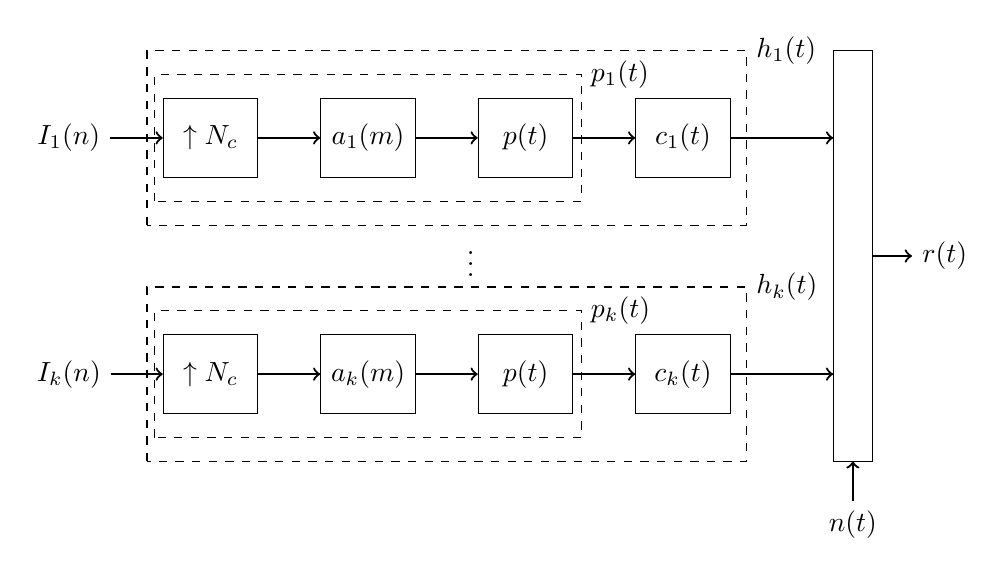
\begin{tikzpicture}
    \node (I1) {$I_1(n)$};
    \node[below of=I1, node distance=3cm] (Ik) {$I_k(n)$};

    \path (I1) -- (Ik) node[midway] (middle) {};

    \node[right of=I1, draw, minimum width=1.2cm, minimum height=1cm, node distance=1.8cm] (up1) {$\uparrow N_c$};
    \node[right of=up1, draw, minimum width=1.2cm, minimum height=1cm, node distance=2cm] (a1) {$a_1(m)$};
    \node[right of=a1, draw, minimum width=1.2cm, minimum height=1cm, node distance=2cm] (p1) {$p(t)$};
    \node[right of=p1, draw, minimum width=1.2cm, minimum height=1cm, node distance=2cm] (c1) {$c_1(t)$};
    \draw[->, thick] (I1) -- (up1);
    \draw[->, thick] (up1) -- (a1);
    \draw[->, thick] (a1) -- (p1);
    \draw[->, thick] (p1) -- (c1);
    \draw[dashed] ([shift={(-.1,-.3)}]up1.south west) rectangle ([shift={(+.1,+.3)}]p1.north east) node[right] {$p_1(t)$};
    \draw[dashed] ([shift={(-.2,-.6)}]up1.south west) rectangle ([shift={(+.2,+.6)}]c1.north east) node[right] {$h_1(t)$};

    \node[right of=Ik, draw, minimum width=1.2cm, minimum height=1cm, node distance=1.8cm] (upk) {$\uparrow N_c$};
    \node[right of=upk, draw, minimum width=1.2cm, minimum height=1cm, node distance=2cm] (ak) {$a_k(m)$};
    \node[right of=ak, draw, minimum width=1.2cm, minimum height=1cm, node distance=2cm] (pk) {$p(t)$};
    \node[right of=pk, draw, minimum width=1.2cm, minimum height=1cm, node distance=2cm] (ck) {$c_k(t)$};
    \draw[->, thick] (Ik) -- (upk);
    \draw[->, thick] (upk) -- (ak);
    \draw[->, thick] (ak) -- (pk);
    \draw[->, thick] (pk) -- (ck);
    \draw[dashed] ([shift={(-.1,-.3)}]upk.south west) rectangle ([shift={(+.1,+.3)}]pk.north east) node[right] {$p_k(t)$};
    \draw[dashed] ([shift={(-.2,-.6)}]upk.south west) rectangle ([shift={(+.2,+.6)}]ck.north east) node[right] {$h_k(t)$};

    \path ([shift={(+.2,+.6)}]c1.north east) -- ++(1.1,0) coordinate (NW);
    \path ([shift={(+.2,-.6)}]ck.south east) -- ++(1.6,0) coordinate (SW);
    \draw[->,thick] (c1) -- (NW |- c1);
    \draw[->,thick] (ck) -- (NW |- ck);
    \draw (NW) rectangle (SW);
    \path (SW) -- (NW |- SW) node[midway] (midsouth) {};
    \draw[<-,thick] (midsouth.center) -- ++(0,-.5) node[below] {$n(t)$};
    \draw[->,thick] (SW |- middle) -- ++(0.5,0) node[right] {$r(t)$};

    \path (I1 |- middle.center) -- (SW |- middle.center) node[midway] {$\vdots$};

\end{tikzpicture}
